
\subsection*{1.}

En faisant le complément à 100 des pourcentages donnés, on peut dresser l'arbre pondéré suivant :

\begin{center}
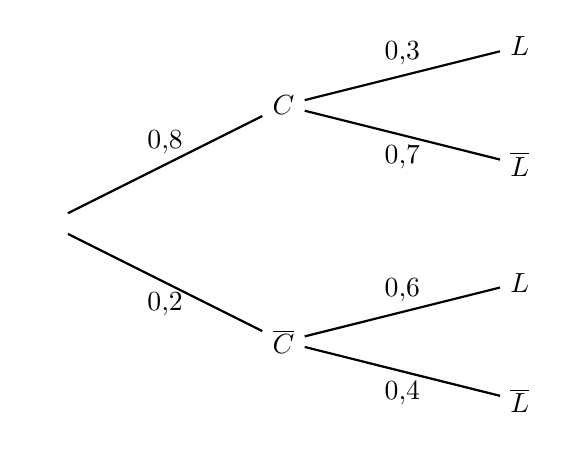
\begin{tikzpicture}[thick, scale=1.5]
\node (P_-1_0) at (-2,-1.5) {$\phantom{A}$};
\node (P_0_0) at (0,-0.5) {$C$};
\draw (P_-1_0) -- (P_0_0) node[midway, above] {$0{,}8$};
\node (P_1_0) at (2,-0) {$L$};
\draw (P_0_0) -- (P_1_0) node[midway, above] {$0{,}3$};
\node (P_1_1) at (2,-1) {$\overline{L}$};
\draw (P_0_0) -- (P_1_1) node[midway, below] {$0{,}7$};
\node (P_0_2) at (0,-2.5) {$\overline{C}$};
\draw (P_-1_0) -- (P_0_2) node[midway, below] {$0{,}2$};
\node (P_1_2) at (2,-2) {$L$};
\draw (P_0_2) -- (P_1_2) node[midway, above] {$0{,}6$};
\node (P_1_3) at (2,-3) {$\overline{L}$};
\draw (P_0_2) -- (P_1_3) node[midway, below] {$0{,}4$};
\end{tikzpicture}
\end{center}

\subsection*{2.}

On a :
\[
P(C \cap L) = P(C) \times P_C(L) = 0{,}8 \times 0{,}3 = 0{,}24.
\]

\subsection*{3.}

On a de même :
\[
P(\overline{C} \cap L) = P(\overline{C}) \times P_{\overline{C}}(L) = 0{,}2 \times 0{,}6 = 0{,}12.
\]
D'après la loi des probabilités totales :
\[
P(L) = P(C \cap L) + P(\overline{C} \cap L) = 0{,}24 + 0{,}12 = 0{,}36.
\]

\subsection*{4.}

\paragraph{a.} D'après la question précédente :
\[
P(X = 4000) = P(L) = 0{,}36,
\]
et par conséquent :
\[
P(X = 2500) = P(\overline{L}) = 1 - 0{,}36 = 0{,}64.
\]

\paragraph{b.} L'espérance de \(X\) est égale à la somme des termes \(n_i \times P_i\), donc :
\[
E(X) = 0{,}36 \times 4000 + 0{,}64 \times 2500 = 1440 + 1600 = 3040.
\]

